\setchapterpreamble[o]{%
  \dictum[Intel Corporation]{``Virtualization is a paradigm shift; it
    changes how you think about your resources.''}}

\chapter{Introduction}
\label{cha:intro}

Virtual machine (VM) technology is a major development in computer systems
design   \cite{buzen73}.     They   have   extended    the   multi-access,
multi-programming  and multi-processing  systems  to be  multi-environment
systems  as well by  providing efficient  ``copies'' of  complete computer
systems \cite{goldberg73}.

Todays  personal   computer  systems   are  powerful  enough   to  provide
virtualization  technology, which  has been  long time  reserved  for high
performance  mainframe  systems. The  paper  \emph{Analysis  of the  Intel
  Pentium's    Ability    to   Support    a    Secure   Virtual    Machine
  Monitor}\cite{robin00analysis}  discusses the  problems  of how  virtual
machines can be efficiently supported by the IA32 architecture.

In  the last few  years, the  remote execution  of applications  gained on
importance, because powerful server systems need not be maintained locally
but  could be  deployed elsewhere.  Grid  middle-wares such  as Globus  or
Unicore  are examples  for environments,  in  which users  can send  their
computation to  some computer  connected to the  grid and get  the results
back.

This work  is about  the execution of  arbitrary applications on  a remote
system exploiting virtual machines. It addresses the problem that multiple
potentially  broken applications  are typically  executed on  remote hosts
side by  side ---  if one application  behaves ``wrong''  (e.~g.~CPU cycle
consumption,  memory  leakage, etc.)  it  may  involve other  applications
running on the same host.

Sharing of computing resources must always consider security, availability
of  the resources and  fairness among  the resource  users.  To  make that
clear,  take  two jobs  from  different users  that  are  scheduled to  be
executed on the  same grid-node with overlapping execution  times. Let one
of the jobs have  a memory leak --- which is not  as uncommon as you might
think --- that task will eventually  eat up all the available memory. This
misbehavior not only  harms the other job, but also  may harm the software
used to connect the host to the grid.

The here  proposed solution is separation using  virtual machines provided
by  the Xen  hypervisor. Each  job  will be  executed in  its own  virtual
machine and  is not  able to harm  either other  jobs running on  the same
physical host, or the physical node itself.

\section{The history of virtualization technologies}
\label{sec:virtualization-history}

The history of virtualization starts  with a paper entitled ``Time sharing
in  large,  fast  computers''  \cite{Strachey59}  written  by  Christopher
Strachey in  1959. His idea bases  on a single-CPU  system which processes
jobs one  after each  other. If  a program blocks  due to  some peripheral
access the  next program in the queue  gets started and will  be run until
the next peripheral  access occurs and so forth.   The system presents the
user with  a \emph{logical CPU} and  a scheduler assigns  this logical CPU
transparently  for   the  user  to   a  physical  CPU.   His   concept  of
``time-sharing''  is now  known  as \emph{\gls{glo:multi-programming}}  as
Christopher Strachey states in a letter to Donald E. Knuth in 1974.

This very simple scheduling strategy maximizes the utilization of the most
worthy resource  to that time  --- the CPU  --- and provides the  base for
current scheduling strategies such as \gls{glo:multi-tasking}.

\subsubsection{The Atlas Project}

Later on  in the  early 1960s,  the ``Atlas project''  --- a  joint effort
between the  University of Manchester and  Ferranti~Ltd.~has been founded.
The Atlas  computer has been the  most powerful mainframe  computer in the
world in  those days.   It provided spooling  mechanisms and  pioneered in
\emph{demand  paging}  and  \emph{supervisor  calls}, they  also  invented
``\gls{glo:virtmem}'' --- called ``one-level store'' in
the Atlas system.

The  supervisor calls  where activated  through interrupt  routines  or by
so-called   \emph{\gls{glo:extracode}}  instructions   within   an  object
program.  Atlas made use of two ``virtual machines'' --- one executing the
\gls{glo:supervisor}  and  the  other   was  used  to  run  user  programs
\cite{virtualization-overview}.

\subsubsection{The M44/44X Project}

The IBM Watson  Research Center has been the home  for the M44/44X Project
in the  mid 1960s. The goal of  this project was to  evaluate the upcoming
concepts of  \gls{glo:time-sharing}.

The research team, led by R.~A.~Nelson, developed a way of partitioning an
IBM 7044 machine into sub-machines that  were each images of the 7044 with
less memory  --- the  main machine was  called M44, the  sub-machines 44X,
thus the project's name \cite{virtualization-overview}.

Especially David  Sayre and Belady made extensive  experimental studies to
evaluate the  performance of  \gls{glo:virtmem}, load control  and various
scheduling policies \cite{Belady66,denning81}.

\subsubsection{IBM virtual machines and the ``virtual machine monitor''}

IBM    has   been   perhaps    the   most    important   force    in   the
\gls{glo:virtualization} area  and a  number of IBM-based  virtual machine
systems were developed: the CP-40  (for a modified version of IBM 360/40),
the CP-67 (for  the IBM 360/67) and of course the  famous VM/370, and many
more.

The  VM/370 is  the name  for three  operating systems,  the \emph{Control
  Program}  (CP),  \emph{Conversational  Monitor  System}  (CMS)  and  the
\emph{Remote Spooling and Communications Subsystem} (RSCS) \cite{creasy81}.
Together they provide a way to form virtual machines, which can be used by
many users. The CP therefore  simulates multiple copies of the hardware on
which it is running.  The CMS is the operating system which runs in such a
``virtual machine'' and provides access for the users.

These  virtual  machines  were   typically  identical  ``copies''  of  the
underlying  hardware. A  special  component called  the ``virtual  machine
monitor''  (\gls{glo:VMM}) ran  directly  on the  real hardware.   Several
virtual machines could then be created using the VMM by assigning parts of
the hardware to the virtual machine. The virtual machine could then run an
operating system on its own and  only had access to those parts configured
through  the VMM.  By  this, new  operating  systems could  be tested  and
developed in a stable and secure manner.

\begin{figure}[htbp]
  \begin{center}
  \begin{minipage}{0.75\textwidth}
    \begin{center}
      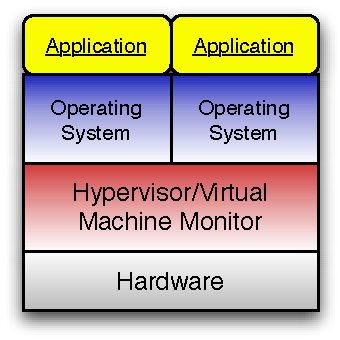
\includegraphics[scale=.75]{architecture-with-virtualization}
    \end{center}
    \caption[Virtualization   architecture]{The   so-called   bare-metal
      virtualization:   A  virtual   machine  monitor   runs   as  small
      ``operating system'' on the  real hardware and provides access for
      virtual machines.}
    \label{fig:arch-virt}
  \end{minipage}
  \end{center}
\end{figure}

This  kind   of  virtualization  is  called   ``full''  or  ``bare-metal''
virtualization  ---  an operating  system  running  in  a virtual  machine
provided by the  VMM thinks it runs on real  hardware. An abstract picture
of such an architecture is shown in Fig.~\ref{fig:arch-virt}.

\section{Virtualization techniques}
\label{sec:techniques}

According   to    the   Church-Turing~Thesis   \cite{church_turing_thesis}
\emph{``Any real-world  computation can  be translated into  an equivalent
  computation involving  a Turing machine.''}, every  computer can simulate
any other computer.

\bigskip

\subsection{Partitioning}
\label{sec:vt-partitioning}

The first virtualization technique  bases on partitioning of the available
hardware \cite{borden89}.   It is available  since the 1960s and  has been
provided  by  two  approaches  ---  a software  approach  and  a  hardware
approach.

\subsubsection{Software partitioning}
\label{sec:softw-part}

The IBM CP/67  has been the first operating  system which provided virtual
machine support, it  was running on the System/360 Model  67 and was first
available in 1967 \cite{borden89}.

As described earlier, the CP gave each user a virtual machine on which the
CMS (a  single user  operating system) was  running and provided  the user
with command processing and information management functions. Each virtual
machine was ``copy'' of the base hardware architecture, it was possible to
run OS/360 in  a virtual machine and ``in fact, even  CP/67 itself was run
"second  level" in a  virtual machine  for the  purposes of  debugging and
testing \cite{borden89}''.

\subsubsection{Hardware partitioning}
\label{sec:hardw-part}

Hardware partitioning is an enhancement over software partitioning and was
introduced  by  the  IBM   \emph{System/370  158  MP}  and  \emph{168  MP}
systems. In 1967,  IBM introduced multiprocessor versions of  Model 65 and
67, which  provided duplexed hardware to achieve  tolerance against single
hardware failures.  By  splitting up the whole system  into two sides, two
separate systems could be created  which ran totally independent from each
other.

\subsection{Emulation}
\label{sec:emulation}

This kind of virtualization  simulates a complete hardware architecture in
all  details. By  that every  operating system  and  therefore application
which has been  developed for that particular application  may be executed
within the emulator. Some examples are:
\begin{itemize}
\item  \emph{Wine \cite{wine}}  --- Wine  is  not quite  an emulator,  but
  nonetheless I put it in this list, too. It emulates the Windows API, but
  executes many functions directly  on the underlying x86 hardware without
  emulating each instruction.
\item \emph{Bochs  \cite{bochs}} --- this  is a very portable  open source
  IA-32 PC emulator.  Each machine  instruction will be interpreted and is
  handled in software.  This emulator may for instance be  used to run x86
  code on a PowerPC platform.
\item  \emph{QEMU  \cite{qemu}} ---  this  is  both  an emulator  and  an
  virtualizer, since  it support  two modes of  operation. As  an emulator
  each instruction  gets interpreted  as it is  the case  of \emph{bochs},
  e.g.~it is possible  to emulate an ARM processor on  your PC. To achieve
  better  performances a  technique called  \emph{dynamic  translation} is
  used.   Running as  a virtualizer,  QEMU is  able achieve  nearly native
  performance, since most of the instructions are directly executed on the
  host CPU --- to make this possible a kernel module (QEMU accelerator) is
  required.
\end{itemize}

There are several software  and hardware solutions available which provide
a  virtualized  platform.

\begin{description}
\item[Emulation] An  emulator simulates the complete hardware  and as such
  allows the execution of unmodified guest operating systems. Examples are
  Bochs and Qemu (without its acceleration techniques) for instance.
\item[Native vir\-tu\-ali\-za\-tion] The  virtual machine in this approach
  simulates just enough hardware to let  an unmodified guest to be run. As
  mentioned earlier,  this field  was pioneered in  the beginnings  of the
  1960s.
\item[Paravirtualization]  In  this case,  the  virtual  machine does  not
  necessarily need to simulate hardware, instead it provides a special API
  to which a guest system has to  be ported. That means one can not run an
  unmodified guest on  top of a paravirtualized machine.  Examples in this
  field include Xen and VMWare ESX Server.
\item[Operating system-level  virtualization] This kind  of virtualization
  uses the same  kernel for the host and all guest  systems --- the guests
  run  ``within''  the  host.   Examples include  Solaris  Containers  and
  Free-BSD Jails.
\item[Application  virtualization] The  Java virtual  machine is  a widely
  known  and used implementation  of this  technique. Programs  written in
  Java are compiled into ``Java byte  code'' which is then executed by the
  Java   runtime   environment   (virtual   machine  plus   an   operating
  environment).  This  approach made it  possible to create  software that
  can  be run  on every  platform for  which a  port of  the  Java virtual
  machine exists.
\end{description}

In this  work I am  dealing with the ``paravirtualization''  technique and
especially with the Xen hypervisor.

\subsection{Problems on x86 hardware}
\label{sec:x86-problems}
\nocite{robin00analysis}

From \cite{popek75}: New architectures are discussed in \cite{goldberg73},
while hardware and software methods  which have been employed for existing
third generation  architectures are described in  \cite{buzen73}. In these
latter cases, the  virtual machine monitor typically is  run in privileged
mode,  and all  other  software in  user  mode. For  this  approach to  be
successful,  all ``sensitive''  instructions must  trap when  execution is
attempted in user mode, so that they can be simulated.




\section{The Xen hypervisor}
\label{sec:xen-hypervisor}

\cite{hendricks79}: ``The term “hypervisor” is applied to computer systems
that present a very basic  user program interface-one which is so nearly
identical to a  particular computer machine interface that  an operating
system intended  to support such machines  may serve as  a hypervisor user
program without  software modification. The user interface  presented by a
hypervisor is commonly called a  virtual machine; the term “subsystem” may
be applied to the complex of software used within a virtual machine.''

Xen  \cite{xen}  is  a  virtualization  technology to  partition  a  given
physical machine into smaller virtual machines (i.e. \gls{glo:VM}s).  Each
of these  \gls{glo:VM}s has their own  main memory, file  space, access to
one or  more virtual CPUs and everything  else that is required  to run an
operating system.   Xen belongs to the hosted  virtualization group, which
means that the \gls{glo:VMM} still requires an operating system to run and
does not represent a stand-alone operating system itself.

\begin{figure}[htbp]
  \begin{center}
    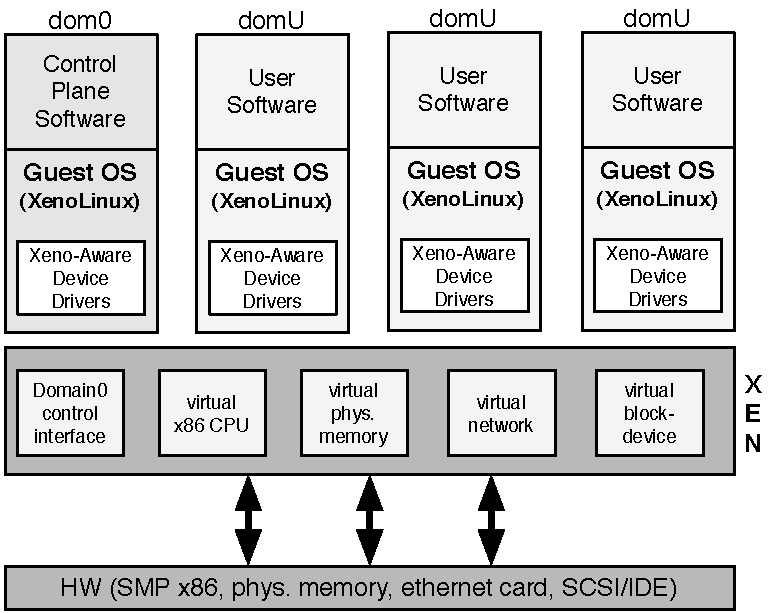
\includegraphics[height=8cm]{xen-architecture}
  \end{center}
  \caption[Xen architecture]{The structure of a system running the Xen
    hypervisor and several user domains (taken from \cite{xen-art})}
  \label{fig:xen-architecture}
\end{figure}

Xen  virtual  machines  (see Fig.~\ref{fig:xen-architecture})  are  called
``domains''  and   the  top-level  or   most  privileged  one   is  called
\texttt{Domain-0}  --- or  \texttt{dom0} for  short ---  this is  the one,
which runs the control and management programs that are required to create
new virtual machines.  The  virtual machine instances beside \texttt{dom0}
are called ``user  domains'' --- or \texttt{domU}s for  short --- they are
less privileged and their access to the hardware is controlled and managed
by the hypervisor running in \texttt{dom0}.

The  operating  system  running  within  a user  domain  accesses  virtual
hardware  provided by  the Xen-architecture  (SCSI or  IDE  controllers to
access virtual hard drives, network interface cards, virtual CPUs, graphic
card device and so on).


\section{Benefits of virtualization}
\label{sec:benefits}

To  satisfy customer  demands,  not a  single,  general purpose  operating
system  can be  used, over  the time  dozens of  specialized  systems have
evolved --- for instance on  consumer desktop systems one can find Apple's
MacOS,  Microsoft   Windows,  some  Linux  distribution   with  a  desktop
environment,  on cluster  systems  or  on systems  which  have to  provide
outstanding  security and availability  typically other  operating systems
are  used   (Linux  for  instance,  may   be  an  exception   due  to  its
adaptiveness).  Each  system has been designed  to address the  needs of a
large segment of the marketplace \cite{borden89}.

\bigskip

The following list are reasons, why multiple operating systems may need to
coexist and  even be used in the  same establishment at the  same time and
how virtual machines fit into that \cite{borden89,virtualization-overview}:

\begin{itemize}
\item  \emph{Diverse Workload}  --- in  large establishments  it  is often
  required, that  different computing  requirements must be  fulfilled. An
  airport, for instance, requires  a highly responsive reservation system,
  a  database system  for aircraft  maintenance  and parts  and a  general
  purpose system for payroll and planning.
\item  \emph{Test  and  development}   ---  many  companies  require  high
  availability and stability of  their computing components, but they also
  may want to test, develop  and deploy new software or software versions.
  
  Here at  the Fraunhofer ITWM,  for instance, SuSE  Linux is used  as the
  operating system for many desktop systems. To provide stability, updates
  have to be tested prior deploying them everywhere.

  The same holds for application  development --- a company will have some
  productive system running the developed application, and this system has
  to be available 24 hours  day. Clearly, development cannot take place on
  the production machines,  since the probability of a  breakage is simply
  too high --- machines solely dedicated for development are required.
\item \emph{Backup  and recovery} --- server  applications which represent
  important  components   for  the  daily   work  (e.g.~database  systems,
  web-servers etc.) must  be available all the time. A  nice thing to have
  in such  a situation  is automatic recovery  from failure ---  to reduce
  down-time two systems can be used: one of them is the productive system,
  the  other one  is a  backup system  that is  an exact  ``copy''  of the
  productive system  and just waits  for a failure  of the other.   Upon a
  system failure  in the  productive system, the  backup system  will take
  over.
\item  \emph{Platform  independent development}  ---  over  the time  many
  different  operating  systems have  evolved  ---  various Unix  flavours
  (FreeBSD, Linux for  instance), DOS, Microsoft Windows, Mac  OS, just to
  name some of them --- not all of them are compatible to each other.

  Application developers who  want to develop an application  that runs on
  several of these operating systems are required to port and verify their
  application on each  target system and maybe on  several versions of the
  same target system.

  One way  is to have  an extra machine  with the target  operating system
  installed on  it just for testing  and porting issues ---  that not only
  imposes energy  costs but also maintenance  costs.

  The other way is to use  virtual machines instead of actual machines ---
  each virtual machine runs a version of a target operating system.
\item  \emph{Server consolidation} ---  a common  approach for  many small
  companies is to have one server on which runs for instance a web server,
  some content management system with a database as its back-end under the
  same  operating system.

  That approach  may involve security problems,  since if just  one of the
  services   contains  a   security  hole,   the  whole   system   can  be
  compromised. Using virtual  machines for each of the  services, the only
  system  that is  now compromised  is the  one providing  this particular
  service.
\end{itemize}


%%% Local Variables: 
%%% TeX-master: "main.tex"
%%% End:
